\section{Theoretical Background}
\label{sec:theoretical_background}
In this chapter we introduce the theoretical background of the machine learning algorithms used throughout this thesis. We explain the different machine learning concepts and the purpose of a classifier. Furthermore, we lay the foundations for the individual build blocks and layers of deep neural network system. We explain the differences between convolutional neural network and recurrent neural networks and follow up by describing hybrid models constructed of both of these. More specifically, we describe the convolutional recurrent neural network (CRNN) architecture as used in this thesis. Finally, we present different representations for audio file suitable for machine learning tasks.

\subsection{Machine Learning}
\todo{more bla bla}
\subsubsection{Types of Machine Learning}
The field of machine learning covers a multitude of different learning algorithms. While each of these is based on a different mathematical foundation they also serve many different purposes. \textit{Classification} algorithms divide their data into two or more distinct classes. Each new input sample can then be assigned to one of these learned classes. For example we could image an app that automatically classifies pictures of food recognizes and names the respective dishes. While classification results are always discrete values a \textit{regression} algorithm outputs continuous values instead. For example image a regressor that predicts the future price of your favorite food based on historical price data. For other purposes it is more important to know which data samples are similar to each other and form a group of their own. \textit{Clustering} algorithms can divide data into groups and unlike with classification these group are usually not know ahead of time. For instance a customer management system could cluster everyone into distinct clusters of different focus groups.

Regardless of an algorithms purpose machine learning can typically divided into three categories from a high level point of view:

	\begin{description}
		\item[Supervised Learning] is the task of building a machine learning model with label training data. Every data sample used during training is a pair consisting of a vector or matrix representation of the data and a label identifying the data as belonging to a certain class. Typically a label is represented as a single number or one-hot encoded vector. Supervised learning algorithms learn a inference function that maps every data sample to its expected output label. A trained model should then be able to infer a suitable output class or value for new unknown data. 
				
		\item[Unsupervised Learning] is the task of building a machine learning model with unlabeled training data. Unlike for supervised learning all training samples do not include a label of the desired model outcome. Unsupervised Learning algorithms learn a function by  detecting the hidden structures inside the data. Many clustering algorithms fall into this category.
		
		\item[Reinforcement Learning] is the task of building a machine learning model without a set of classical training data. Instead a reinforcement learning system is set within a specific environment and executes a set of actions. Each action's effect on the environment is measured and reward is calculated. This rewards maximizes the training of the system to find some actions or a sequence of actions to be effective towards achieving a goal. This setup is similar to simulations in some ways. 
	\end{description}

The system described in this thesis is a supervised classification approach using a large scale labeled training dataset.

\subsubsection{Classification}
Classification in the context of machine learning refers to task of assigning a data sample to a class. Classification algorithm are a form of supervised learning and hence need a training dataset of labeled data. The input to classifier are referred to as \textit{features}. Classical machine learning algorithms such as support vector machine (\ac{svm}) or a linear classifier usually require input features carefully designed by a domain expert to be a good representation of the original problem. This process is often referred to as \textit{feature engineering}. In contrast, deep learning classifiers such as \textit{neural networks} are able to directly work on the raw data representations. This has the benefit to build machine learning systems without the need for a domain expert but comes at the price of increased computation requirements. For computer vision tasks, for example, it used to be customary to train classical systems on preprocessed and extracted features of an images such as SIFT key points\cite{lowe1999object} or HOG descriptors\cite{dalal2005histograms}. Deep learning systems, on the other hand, are capable of processing the complete raw pixels of the input image.

	\begin{figure}[]
  		\centering
    	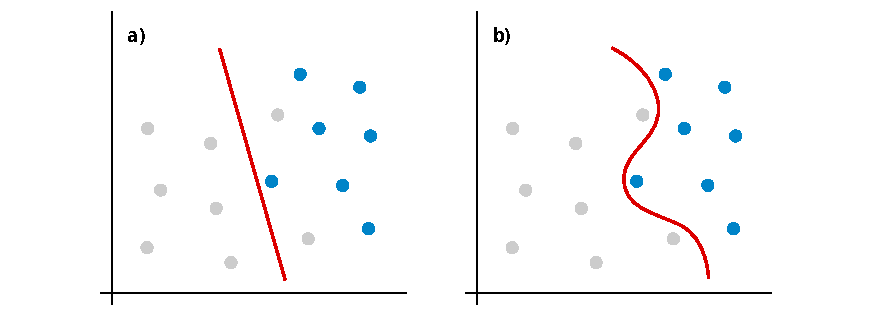
\includegraphics[width=\textwidth, keepaspectratio]{img/classifiers.pdf}
    	\caption{An example of two classifiers: A linear classifier (a) divides the data using a straight line but misclassifies two data points. A neural network (b) is able to learn a more complex decision boundary and separates the dataset without errors.}
    	\label{fig:classifiers}
	\end{figure}

Figure \ref{fig:classifiers} shows an example of two binary classifiers divide a simple dataset into two classes in 2D space. On the left-hand side is linear classifier dividing all points along a straight line. While this sort of classifier is very easy to train and understand it lacks the necessary foundation to divide more complex datasets. On the right-hand side is a neural network (more details in the next section) featuring a more complex, yet more accurate decision boundary. 

\subsection{Building Blocks of Deep Neural Networks}


\subsubsection{Fully Connected Layer}
\subsubsection{Convolutional Layers}
\subsubsection{Pooling Layers}
\subsubsection{Batch Normalization Layers?}
\subsubsection{Softmax Loss Function}

\subsection{Recurrent Neural Networks}
\subsubsection{Long Short Term Memory Networks}

\subsection{Hybrid Networks}
\label{sec:hybrid_networks}

	\begin{figure}[]
  		\centering
    	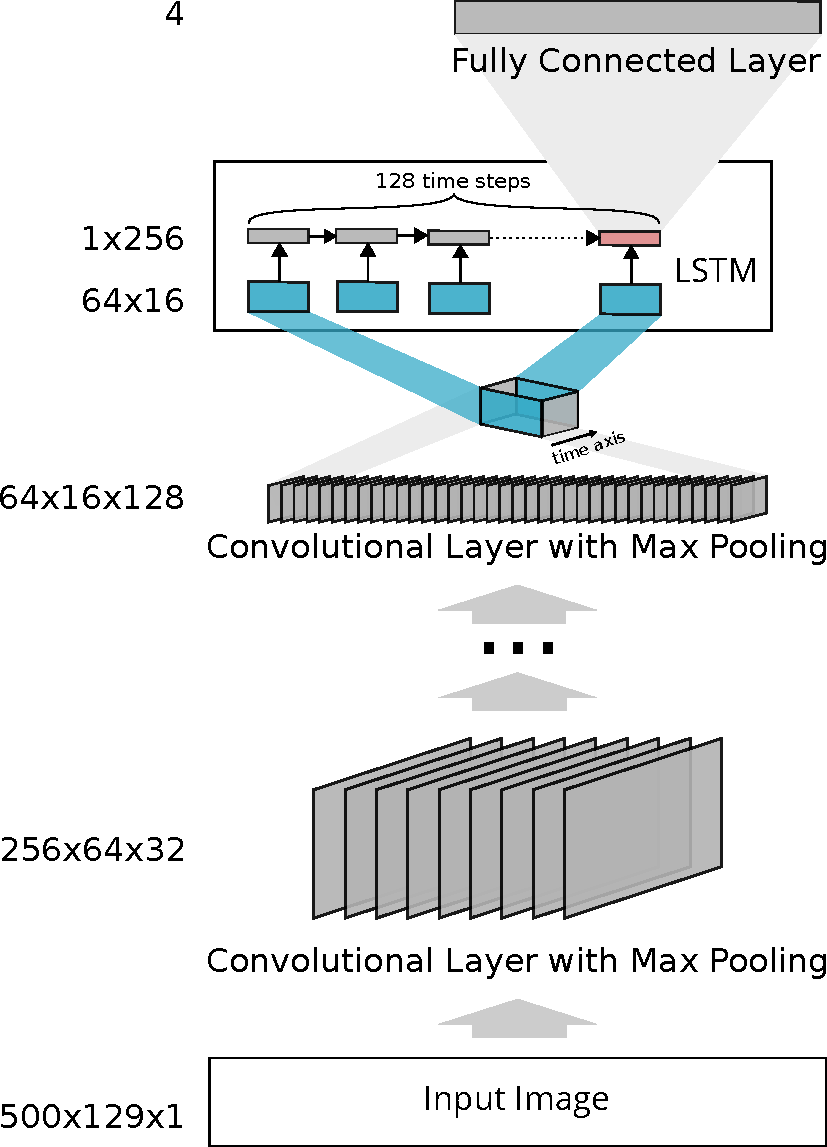
\includegraphics[width=\textwidth, keepaspectratio]{img/crnn.pdf}
    	\caption{Our proposed CRNN hybrid network architecture consists of two networks. A CNN transforms our input images into an intermediary representation of our audio frequencies. The 3D output of final convolutional layer of the CNN is sliced along the x-axis (time axis) into 2D time steps still containing all feature map information. The output of the final LSTM time step is fed into a fully connected layer for classification.}
    	\label{fig:crnn}
	\end{figure}
	
	\begin{figure}[]
  		\centering
    	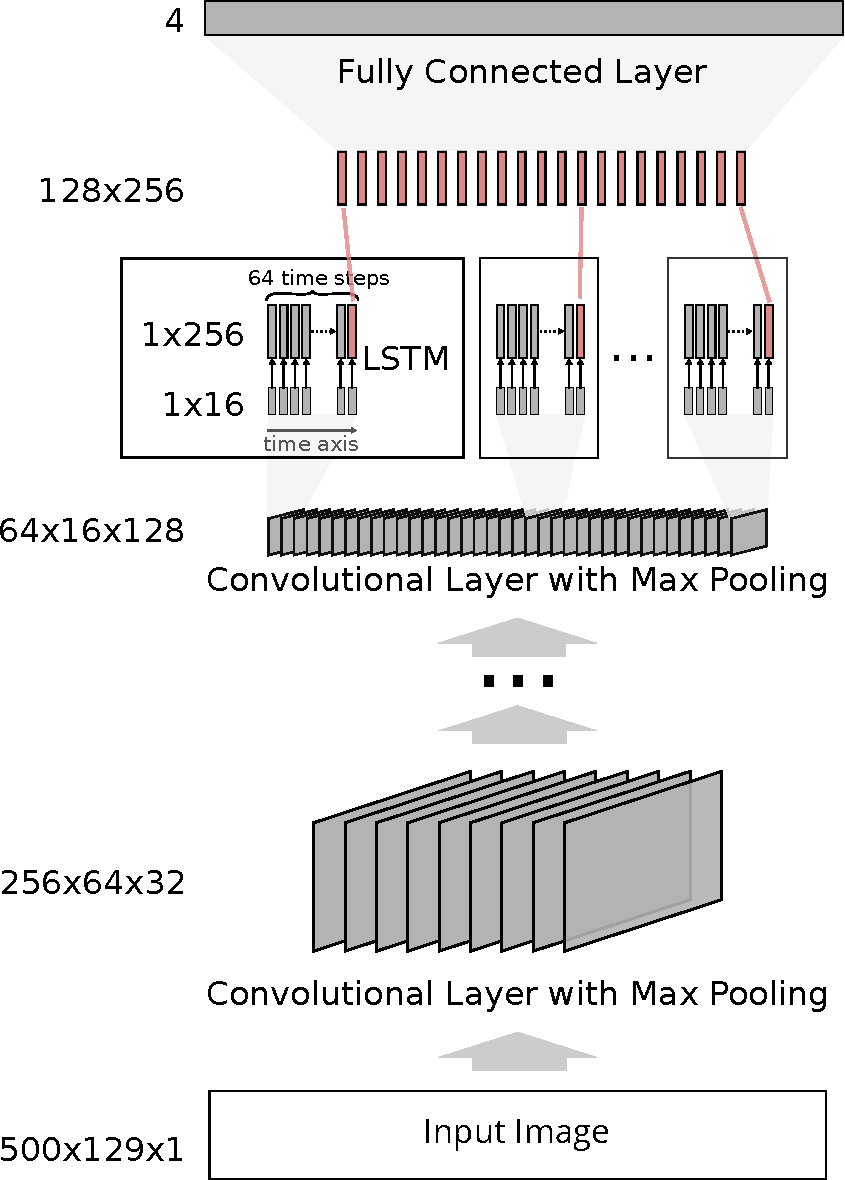
\includegraphics[width=\textwidth, keepaspectratio]{img/crnn2.pdf}
    	\caption{An alternative approach for a hybrid CRNN network. Each single feature map of the final convolutional layer is fed to separate LSTM networks as a 2D input. Each LSTM interprets the vector entries along the x-axis as time steps and operates on thin slice of the data. The output of the final time step of each LSTM is concatenated into a single vector serving as the input to a fully connected classification layer.}
    	\label{fig:crnn}
	\end{figure}

    \begin{itemize}
        \item Convolutional Recurrent Neural Networks
        \item What is their purpose? Averaging over predictions / majority voting
    \end{itemize}

\subsection{Audio Representations}
\label{sec:audio_representations}
    \begin{itemize}
        \item MFCC
        \item Spectrogram (harmonics, formants)
        \item https://home.cc.umanitoba.ca/~robh/howto.html
        \item Waveform
        \item Mel-scale
        \item frequency --> phoneme --> word --> sentence --> language
    \end{itemize}